\section{Kinematics for the Geomagic touch}

As shown on \figref{fig:phantom_omni}, the Phantom omni has 6 joints, from which the kinematic tabel shown on \tabref{tab:kin_geo} can be dereived. 

\begin{table}[h!]
\centering
\begin{tabular}{|l|l|l|l|l|}
\hline
 $j_i$ 	  & $a_i$    & $d_i$ & $\alpha_i$ 		 & $\theta_i$ 			 \\ \hline
 1  	  &  $0$     & $d_1$ & $\frac{\pi}{2}$	 & $q_1$ 			     \\ \hline
 2  	  &  $a_2$   & $0$ 	 & $0$ 		 		 & $q_2 + \theta_1$ 	 \\ \hline
 \rom{1}  &  $0$	 & $0$ 	 & $\frac{\pi}{2}$ 	 & $\frac{\pi}{2} + q_3$ \\ \hline
 3  	  &  $0$	 & $d_3$ & $0$ 		 		 & $0$ 					 \\ \hline
 4  	  &  $0$	 & $d_4$ & $\frac{\pi}{2}$ 	 & $\pi + q_4$ 			 \\ \hline
 \rom{2}  &  $0$	 & $0$ 	 & $\frac{\pi}{2}$   & $\pi +q_5$ 			 \\ \hline
 5  	  &  $0$	 & $d_5$ & $0$ 		 		 & $0$ 	 				 \\ \hline
 %6  	  &  $0$	 & $d_6$ & $\theta$ 		 & $q_6$ 				 \\ \hline
\end{tabular}
\caption{Tabular which contain the kinematics for the Geomagic touch described in \secref{sec:geo_magic}.The Roman numbers defines the fictional joints}
\label{tab:kin_geo}
\end{table}



\begin{figure}[H]
	\centering
	\scalebox{0.75}{
	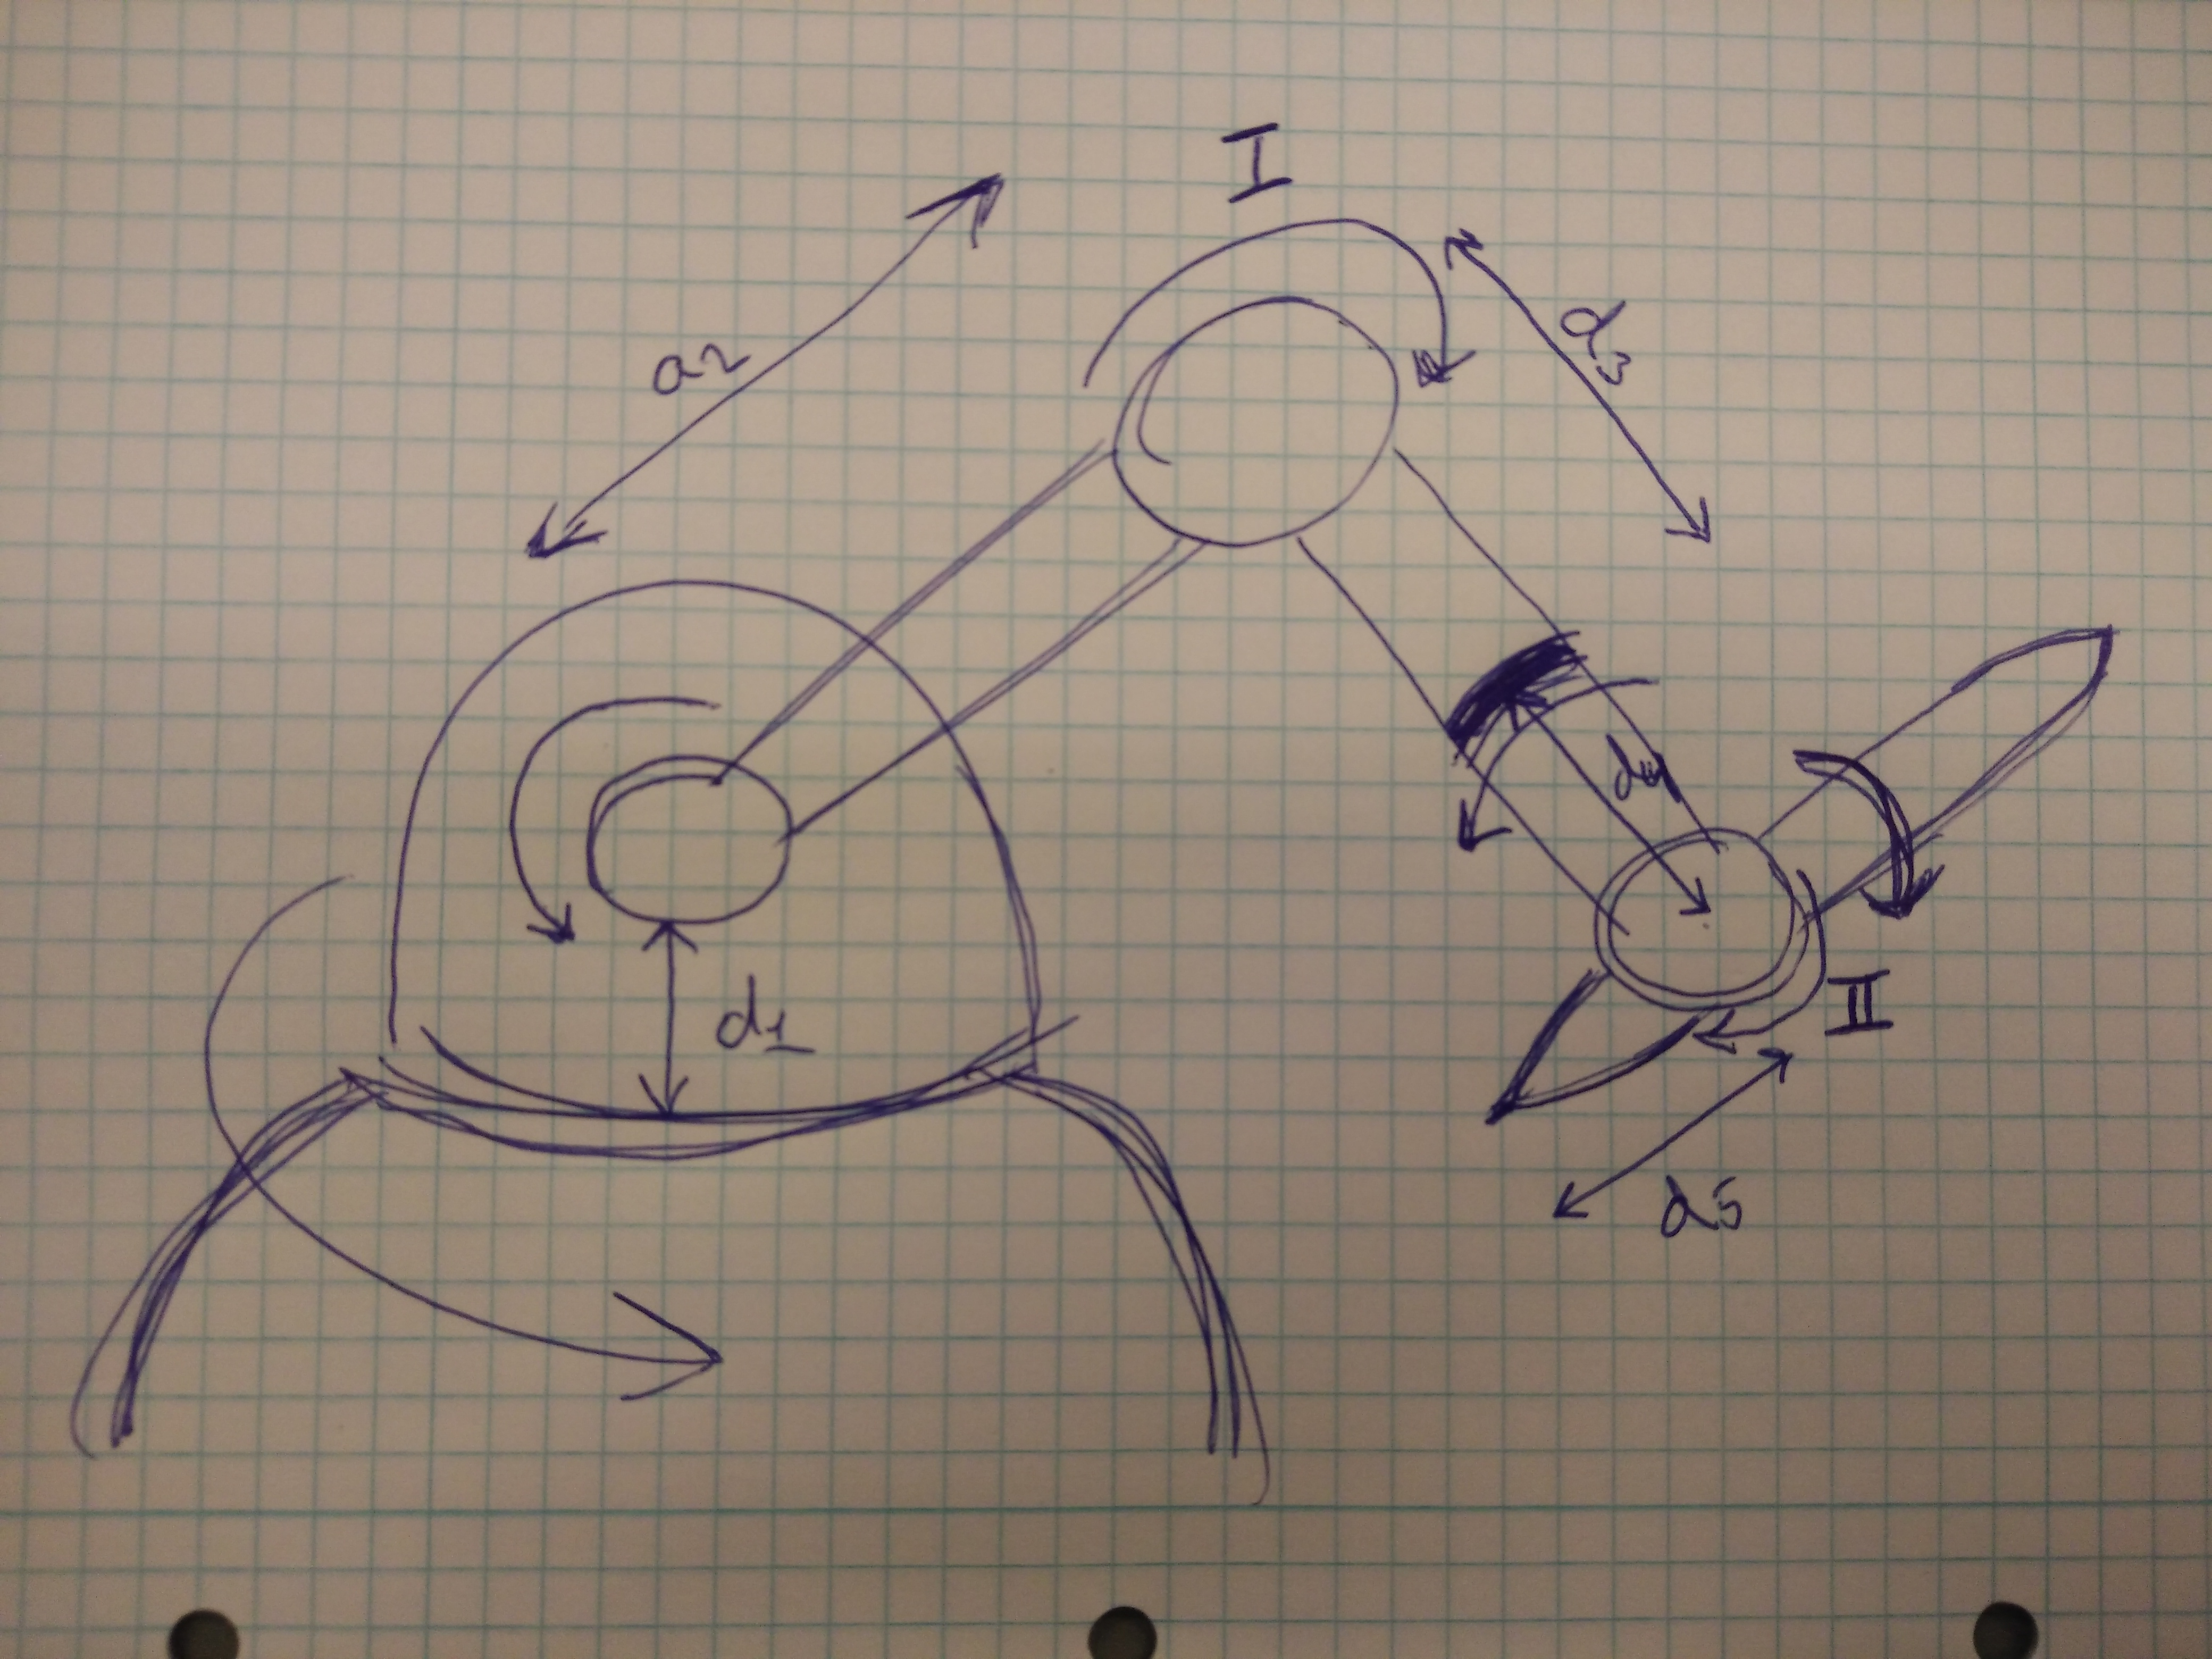
\includegraphics[width=\linewidth]{Fast_draw_Kino.jpg}}
	\caption{Overview of the Phantom omni's first three joints.}
	\label{fig:phantom1}
\end{figure}


